\documentclass{beamer}

\usetheme{LMU}

\usepackage[utf8]{inputenc}
\usepackage[T1]{fontenc}

\usepackage[german]{babel}

\usepackage{amssymb, amsmath, amsfonts, enumerate}
%\usepackage{bbold}
\newcommand\hmmax{0}
\usepackage{bm}
%\usepackage{dsfont}
\usepackage{pxfonts}
\usepackage{xcolor}

\usepackage{tikz}
\usetikzlibrary{%
   arrows,%
   calc,%
   fit,%
   patterns,%
   plotmarks,%
   shapes.geometric,%
   shapes.misc,%
   shapes.symbols,%
   shapes.arrows,%
   shapes.callouts,%
   shapes.multipart,%
   shapes.gates.logic.US,%
   shapes.gates.logic.IEC,%
   er,%
   automata,%
   backgrounds,%
   chains,%
   topaths,%
   trees,%
   petri,%
   mindmap,%
   matrix,%
   calendar,%
   folding,%
   fadings,%
   through,%
   patterns,%
   positioning,%
   scopes,%
   decorations.fractals,%
   decorations.shapes,%
   decorations.text,%
   decorations.pathmorphing,%
   decorations.pathreplacing,%
   decorations.footprints,%
   decorations.markings,%
   shadows}
%\usepackage{bbold}
\usepackage{hyperref}

\setbeamertemplate{blocks}[rounded][shadow=true]
\definecolor{lmugreen2}{RGB}{0,120,94}
%\definecolor{lmugreen2}{RGB}{0,148,64}
\definecolor{lmugreen}{RGB}{0,140,84}
\definecolor{unidurham}{RGB}{126,49,123}

\parindent0pt
\setlength{\unitlength}{1ex}
\setlength{\fboxsep}{0ex}

\def\then{{\color{lmugreen}$\rule[0.35ex]{2ex}{0.5ex}\!\!\!\blacktriangleright$}}
%\def\then{{\color{lmugreen}$\blacktriangleright\!\blacktriangleright$}}
%\def\then{{\color{lmugreen}$\blacktriangleright$}}
%\def\then{{\color{lmugreen}$\Rrightarrow$}}
%\def\then{{\color{lmugreen}$\rhd$}}
%\def\then{{\color{lmugreen}$\gg\!\!\!\!\!\gg$}}
%\def\then{{\color{lmugreen}${\mathbf{\gg}}$}}
\def\play{{\color{lmugreen}$\blacktriangleright$}}

\def\rthen{{\color{lmugreen}$\rule[0.35ex]{0.5ex}{0.95ex}\rule[0.35ex]{1.3ex}{0.5ex}\!\!\!\blacktriangleright$}}

\def\thenthen{{\color{lmugreen}$\blacktriangleleft\!\!\!\rule[0.35ex]{2ex}{0.5ex}\!\!\!\blacktriangleright$}}

\def\gplus{{\color{lmugreen}\rule[0.45ex]{1.4ex}{0.4ex}\hspace{-0.9ex}\rule[0.0ex]{0.4ex}{1.3ex}\hspace{0.5ex}}}
\def\gminus{{\color{lmugreen}\rule[0.45ex]{1.4ex}{0.4ex}}}


\def\blau#1{{\color{lmugreen2}#1}}
\def\rot#1{{\color{red}#1}}
\def\gruen#1{{\color{blue}#1}}
%\def\gruen#1{{\color{gray}#1}}

%%%%%%%%%%%%%%%%%%%%%%%%%%%%%%%%%%%%%%%%%
%% Definitions & shortcuts for thesis  %%
%%%%%%%%%%%%%%%%%%%%%%%%%%%%%%%%%%%%%%%%%

\def\pdc{prior-data conflict}

\newcommand{\reals}{\mathbb{R}}

\newcommand{\dd}{\,\mathrm{d}}

\newcommand{\mbf}[1]{\mathbf{#1}}

\newcommand{\X}{\mbf{X}}
\newcommand{\x}{\mbf{x}}

\def\yzr{\rot{\yz}}
\def\ynr{\rot{\yn}}
\def\byzr{\rot{\byz}}
\def\bynr{\rot{\byn}}
\def\yzor{\rot{y\uz_1}}
\def\yzjr{\rot{y\uz_j}}
\def\yzkr{\rot{y\uz_k}}
\def\yzlr{\rot{\yzl}}
\def\yzur{\rot{\yzu}}
\def\ynlr{\rot{\ynl}}
\def\ynur{\rot{\ynu}}
\def\yzjlr#1{\rot{\ul{y}\uz_#1}}
\def\yzjur#1{\rot{\ol{y}\uz_#1}}


\def\nzg{\gruen{\nz}}
\def\nng{\gruen{\nn}}
\def\nzlg{\gruen{\nzl}}
\def\nzug{\gruen{\nzu}}
\def\nnlg{\gruen{\nnl}}
\def\nnug{\gruen{\nnu}}

\def\psib{\blau{\psi}}
\def\bpsib{\blau{{b}(\psi)}}


% ------------ shading start
\newsavebox{\tempbox}
\newcommand\leftrightshading[3]{%
  \begin{tikzfadingfrompicture}[name=inputtext]
    \node [text=white] {#1};
  \end{tikzfadingfrompicture}
  \begin{lrbox}{\tempbox}%
    \begin{tikzpicture}
      \node [text=white,inner sep=0pt,outer sep=0pt] (textnode) {#1};
      \shade[path fading=inputtext,fit fading=false,left color=#2,right color=#3]
      (textnode.south west) rectangle (textnode.north east);
    \end{tikzpicture}%
  \end{lrbox}
  % Now we use the fading in another picture:
  \usebox\tempbox{}%
}
% ------------ shading end


%\def\PZc{\mathrm I\!\Pi\uz}
\def\PZc{\leftrightshading{$\mathrm I\!\Pi\uz$}{blue}{red}}
\def\PNc{\PN}


\title[Bayesian Inference with Sets of Conjugate Priors]
{Bayesian Inference with Sets of Conjugate Priors: Parameter Set Shapes and Model Behaviour}

\author%[]
       {Gero Walter}

\institute{Department of Statistics\\
           Ludwig-Maximilians-Universit\"at M\"unchen (LMU)\\
                      {}%\{gero.walter; thomas\}@stat.uni-muenchen.de
}

\date{March 6th, 2013}


\titlegraphic{
%\begin{center}

\includegraphics[scale=0.032]{lmu_logos/lmu_massiv.png}
\raisebox{1.375cm}{
\includegraphics[scale=0.4]{lmu_logos/lmu_statistic.pdf}
}
%\end{center}
}

\begin{document}


\frame{
\titlepage
}

\frame{\frametitle{Outline}
\begin{enumerate}
\item Common-cause failure modelling
\item Bayesian inference with sets of priors
\item Parameter set shapes
\end{enumerate}
}


\section{Common-cause Failure Modelling}


\frame{
\frametitle{Common-Cause Failures}

\begin{center}
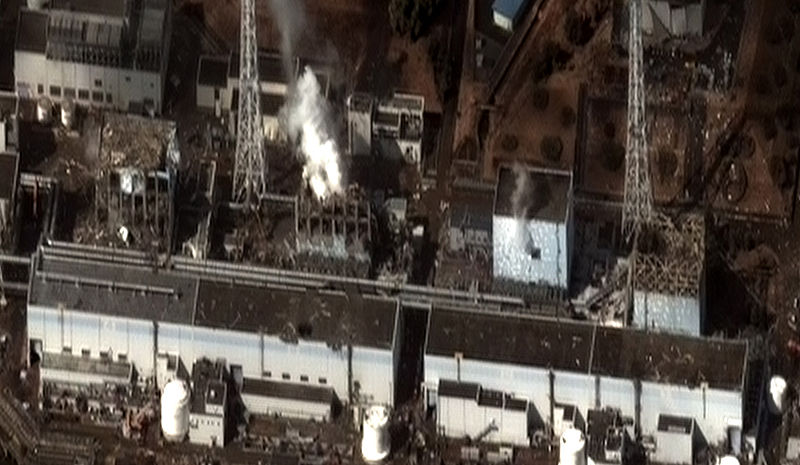
\includegraphics[scale=0.4]{./graph/800px-Fukushima_I_by_Digital_Globe.jpg}\\%[-1ex]
{\tiny Source: Wikimedia Commons, \url{http://commons.wikimedia.org/wiki/File:Fukushima_I_by_Digital_Globe.jpg}}
\end{center}
}


\frame{
\frametitle{Common-Cause Failures}

\begin{itemize}
\item Reliability of redundant systems (emergency diesel generators)
\item Usually 2 -- 4 generators per reactor
\item Sufficient cooling of core if one generator works
%\item Reliability through redundancy is jeopardised by common-cause failure:%\\
\item Redundant components may not fail independently:
 \begin{center}
 \begin{minipage}{0.8\textwidth}
 \begin{alertblock}{common-cause failure} 
 \emph{simultaneous failure of several redundant components\\ due to a common or shared root cause}
 \end{alertblock}
 \end{minipage}
 \end{center}
\item All 12 generators (for 6 reactors) at Fukushima Daiichi\\ were not available due to flooding of machine rooms\\
(Tsunami from T\={o}hoku earthquake)
\item Include common-cause failures in overall system reliability analysis
\end{itemize}
}


\frame{
\frametitle{Common-Cause Failure Modelling}

\begin{columns}%[T]
\begin{column}{0.7\textwidth}\centering
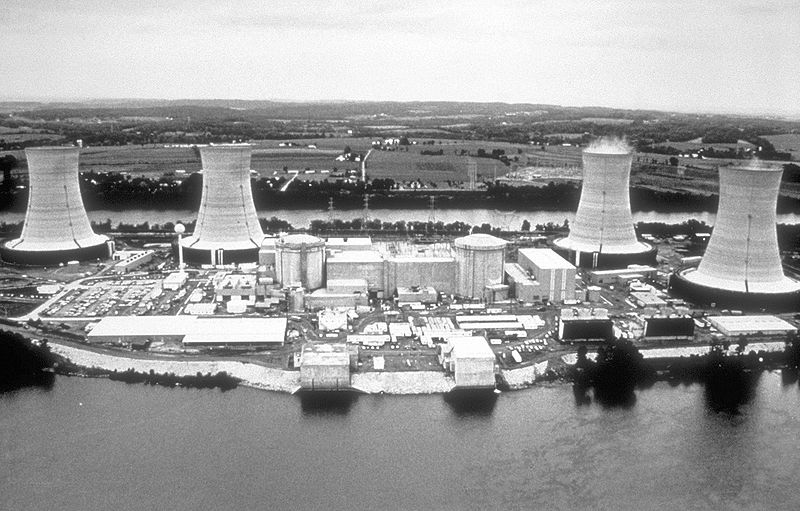
\includegraphics[scale=1.2]{./graph/800px-Three_Mile_Island_nuclear_power_plant.jpg}
\end{column}
\begin{column}{0.35\textwidth}\centering
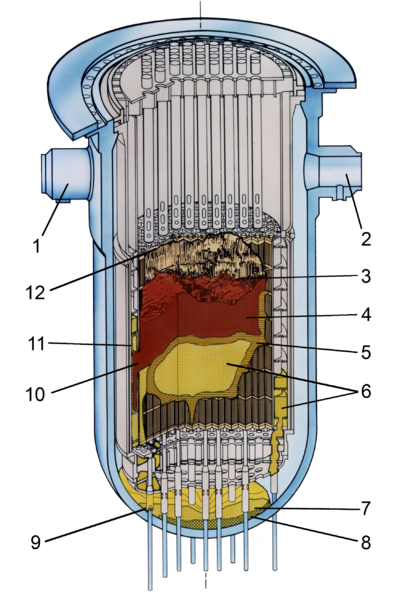
\includegraphics[scale=0.95]{./graph/Graphic_TMI-2_Core_End-State_Configuration.png}
\end{column}
\end{columns}
\vspace*{1ex}
\begin{tiny}
Above: CDC, \url{http://phil.cdc.gov/phil/} ID 1194\\[1ex]
Right: Wikimedia Commons,\\[-1.8ex]
\url{http://commons.wikimedia.org/wiki/File:Graphic_TMI-2_Core_End-State_Configuration.png}
\end{tiny}
}

\subsection{Alpha-Factor Model}

\begin{frame}{Alpha-Factor Model: Definition}
  \begin{block}{Alpha-Factor Model} %\cite{1988:mosleh::common:cause}]
    Multinomial distribution $\mult(\vec{n}\mid\vec{\alpha})$ for common-cause failures \\
    in a $k$-component system\vspace*{-2ex}
    %the number of redundant components in the common-cause component group
    \begin{align*}
      p(\vec{n}\mid\vec{\alpha})=\prod_{j=1}^k\alpha_j^{n_j}\\[-5ex]
    \end{align*}
    where
    \begin{itemize}
    \item \alert{alpha-factor}
      $\alpha_j\coloneqq$
      \parbox[t]{0.6\textwidth}{%
        probability of $j$ of the $k$ components \\
        failing due to a common cause \\
        given that failure occurs
      }
    \item \alert{failure count}
      $n_j\coloneqq$ corresponding number of failures observed
    \item $\vec{n}$ denotes $(n_1,\dots,n_k)$ and $\vec{\alpha}$ denotes $(\alpha_1,\dots,\alpha_k)$
    \end{itemize}
  \end{block}
  (the model actually serves to estimate failure \emph{rates},\\ but the above is all what matters in this talk)
\end{frame}

\begin{frame}{Alpha-Factor Model: Inference ***raus??***}
  \begin{block}{Inference}
    involves rational functions \\
    of probabilities $\vec{\alpha}$ of common-cause failures\\
    and of total failure rate $q_t$ for individual components
  \end{block}
  \begin{center}
    \textbf{this talk: focus on $\vec{\alpha}$ only}
  \end{center}
\end{frame}

\begin{frame}{Alpha-Factor Model: Parameter Estimation}
  \begin{exampleblock}{The Good News}
    attractive feature of this model: \\
    $\vec{\alpha}$ can be estimated directly from data, e.g.\ MLE:
    \begin{align*}
      \alpha_j &= \frac{n_j}{n},\qquad \text{where $\textstyle\sum_{j=1}^n n_j$}
    \end{align*}
  \end{exampleblock}
  \begin{alertblock}{The Bad News}
    \begin{itemize}
    \item typically, for $j\ge 2$, the $n_j$ are very low \\
      with zero being quite common for larger $j$
    \item zero counts = flat likelihoods \\
      standard techniques such as MLE can struggle \\
      to produce sensible inferences for this problem
    \end{itemize}
  \end{alertblock}
  \vspace*{-1ex}
  \begin{center}
    \textbf{\then\ need to rely on \alert{epistemic information}}
  \end{center}
\end{frame}

\subsection{Bayesian Analysis}

\begin{frame}{Bayesian Analysis: Dirichlet Prior}
  $\vec{\alpha}$ considered as uncertain parameter on which we put\dots
  \begin{block}{Dirichlet Distribution}
  \begin{columns}
  \begin{column}{0.65\textwidth}
    \begin{align*}
      p(\vec{\theta}\mid \nzg,\byzr) \propto \prod_{j=1}^k\theta_j^{\nzg\yzjr-1}
    \end{align*}
  \end{column}  
  \begin{column}{0.35\textwidth}
    \rule{0ex}{3ex}where $(\nzg, \byzr)$\\ are \emph{hyperparameters}
 \end{column}
 \end{columns}\vspace*{-1.8ex}
    \begin{align*}
      \nzg &> 0\\[-1ex]
      \byzr &\in \Delta=\Big\{
        (\yzor,\dots,\yzkr)\colon \yzor\ge0,\dots,\yzkr\ge 0,\,\sum_{j=1}^k \yzjr=1
      \Big\}
    \end{align*}
  \end{block}
  \vspace*{-0.5ex}
  \begin{block}{Interpretation}
    \begin{itemize}
    \item $\byzr$ = \alert{prior expectation of $\vec{\alpha}$}, i.e., a prior guess for $\frac{n_j}{n}$ %, $j=1,\ldots,n$
    \item $\nzg$ = determines \alert{spread} and \alert{learning speed} (see next slide)
    \end{itemize}
  \end{block}
\end{frame}

\begin{frame}{Bayesian Analysis: Dirichlet Posterior}
  \begin{itemize}
  \item posterior density for $\vec{\alpha}$ is again Dirichlet
    \begin{align*}
      p(\vec{\alpha}\mid\nzg,\byzr,\vec{n})
%      =:
%      p(\vec{\alpha}\mid\nng,\bynr)
      \propto
      \prod_{j=1}^k\alpha_j^{\nzg\yzjr+n_j-1}.
    \end{align*}
  \item posterior expectation of $\alpha_j$
    \begin{align*}
      %\label{eq:dirichlet:posterior:predictive}
      %\colorbox{red!10!white}{$\displaystyle
      \E[\alpha_j\mid\nzg,\byzr,\vec{n}]
      &=
      \int_{\Delta}\alpha_j p(\vec{\alpha}\mid\nzg,\byzr,\vec{n})\dd\vec{\alpha} \\
      &=
      %\frac{n_j+st_j}{N+s}
      %=
      %\textcolor{green!50!black}{\frac{N}{N+s}}
      %\textcolor{blue}{\frac{n_j}{N}}
      %+
      %\textcolor{green!50!black}{\frac{s}{N+s}}
      %\textcolor{blue}{t_j}
      \colorbox{lmugreen!10!white}{$\displaystyle
      \frac{\nzg}{\nzg+n} \cdot \yzjr + \frac{n}{\nzg+n} \cdot \frac{n_j}{n}
      $}
    \end{align*}
    where $n=\sum_{j=1}^k n_j$ is total number of observations
  \end{itemize}
  %\vspace{1em}
  \begin{center}
    \textbf{we will focus on $\E[\alpha_j\mid\nzg,\byzr,\vec{n}]$} \\
    (in a decision context, this expectation would typically end up \\
    in expressions for expected utility)
  \end{center}
\end{frame}

%\subsection{Example}

\begin{frame}{Example: Prior and Data}
  (taken from Kelly \& Atwood, 2011) %\cite{2011:kelly:atwood})

  \begin{example}
    Consider a system with four redundant components ($k=4$). \\
    %The probability of
    %$j$ out of $k$ common-cause failures, given that failure has happend,
    %was denoted by $\theta_j$.
    The analyst specifies
    the following prior expectation $\mu_{\text{spec},j}$
    for each $\alpha_j$:
    \begin{align*}
      %\label{eq:example:muspec}
      \mu_{\text{spec},1}&=0.950
      &
      \mu_{\text{spec},2}&=0.030
      &
      \mu_{\text{spec},3}&=0.015
      &
      \mu_{\text{spec},4}&=0.005
    \end{align*}
    We have 36 observations, in which 35 showed one component failing,
    and 1 showed two components failing:
    \begin{align*}
      n_1&=35
      &
      n_2&=1
      &
      n_3&=0
      &
      n_4&=0
    \end{align*}
  \end{example}
\end{frame}

\begin{frame}{Example: Non-Informative Priors}
  \alert{large variation in posterior under different non-informative priors} \\
  \begin{itemize}
  \item with constrained maximum entropy prior (Kelly and Atwood, 1996): %\cite{1996:atwood,2011:kelly:atwood}):
    \begin{align*}
      \E[\alpha_1\mid\nzg,\byzr,\vec{n}]&=0.967
      &
      \E[\alpha_2\mid\nzg,\byzr,\vec{n}]&=0.028
      \\
      \E[\alpha_3\mid\nzg,\byzr,\vec{n}]&=0.003
      &
      \E[\alpha_4\mid\nzg,\byzr,\vec{n}]&=0.001
    \end{align*}
  \item 
  with uniform prior $\yzjr=0.25$ and $\nzg=4$:
  \begin{align*}
    \E[\alpha_1\mid\nzg,\byzr,\vec{n}]&=0.9
    &
    \E[\alpha_2\mid\nzg,\byzr,\vec{n}]&=0.05
    \\
    \E[\alpha_3\mid\nzg,\byzr,\vec{n}]&=0.025
    &
    \E[\alpha_4\mid\nzg,\byzr,\vec{n}]&=0.025
  \end{align*}
  \item
  with Jeffrey's prior $\yzjr=0.25$ and $\nzg=2$:
  \begin{align*}
    \E[\alpha_1\mid\nzg,\byzr,\vec{n}]&=0.9342
    &
    \E[\alpha_2\mid\nzg,\byzr,\vec{n}]&=0.0395
    \\
    \E[\alpha_3\mid\nzg,\byzr,\vec{n}]&=0.0132
    &
    \E[\alpha_4\mid\nzg,\byzr,\vec{n}]&=0.0132
  \end{align*}
  \end{itemize}
  % The degree of variation in the posterior under different priors
  % is evidently somewhat alarming.
  % In the next section, we aim to robustify the model
  % by using sets of priors from the start.
\end{frame}

\subsection{Imprecise Dirichlet Model}

\begin{frame}{Imprecise Dirichlet Model: Definition}
\begin{block}{Imprecise Dirichlet Model (IDM) for Common-Cause Failure}
use a \alert{set of hyperparameters}
    % \cite[p.~224, \S 5.4.3]{1991:walley} \cite[p.~32, \S 6]{1996:walley::idm},
    %\cite{1991:walley,1996:walley::idm}
    (Walley 1991, 1996):
    \begin{align*}
      %\label{eq:hyperparams:boxmodel}
      %\mathcal{H}
      \PZc
      =
      \left\{
        (\nzg,\byzr)
        \colon
        \nzg\in[\nzlg,\nzug],\,
        \byzr\in\Delta,\,
        \yzjr\in[\yzjlr{j},\yzjur{j}]
      \right\}
    \end{align*}
\end{block}
\begin{block}{Interpretation}
\begin{itemize}
  \item we are doing a \alert{sensitivity analysis} (\'a la robust Bayes) over $(\nzg,\byzr) \in \PZc$
  \item we take a \alert{set of priors} $\text{conv}\big(\big\{p(\alpha\mid\nzg,\byzr) \colon (\nzg,\byzr) \in \PZc\big\}\big)$
  as model for prior information
%  (resp.\ all convex mixtures of them)
\end{itemize}
\end{block}
Analyst has to specify \\
    bounds $[\nzlg,\nzug]$ and
    bounds $[\yzjlr{j},\yzjur{j}]$ for each $j\in\{1,\dots,k\}$ %\\
\end{frame}

\begin{frame}{Imprecise Dirichlet Model: Elicitation}
  \begin{itemize}
  \item   $[\yzjlr{j},\yzjur{j}]$? Cautious interpretation of prior specifications $\mu_{\text{spec},j}$:
  \begin{align*}
    [\yzjlr{1},\yzjur{1}]&=[0.950,1]
    &
    [\yzjlr{2},\yzjur{2}]&=[0,0.030]
    \\
    [\yzjlr{3},\yzjur{3}]&=[0,0.015]
    &
    [\yzjlr{4},\yzjur{4}]&=[0,0.005]
  \end{align*}
  \item  $[\nzlg,\nzug]$? Good (1965): \\ %\cite{1965:good}: \\
    \begin{center}
    reason about posterior expectations of hypothetical data
    \end{center}
  \end{itemize}
  \begin{alertblock}{}
    $\nzug$ = number of one-component failures required \\
    to reduce the upper probabilities of multi-component failure by half
  \end{alertblock}
  \begin{alertblock}{}
    $\nzlg$ = number of multi-component failures required \\
    to reduce the lower probability of one-component failure by half
  \end{alertblock}
\end{frame}

\begin{frame}{Imprecise Dirichlet Model: Elicitation}
  Reasonable values in example:
  \begin{itemize}
  \item
    $\nzlg=1$: \\
    immediate multi-component failure
    \\
    \then\ keen to reduce lower probability for one-component failure
  \item 
    $\nzug=10$: \\
    after observing $10$ one-component failures \\
    \then\ halve upper probabilities of multi-component failures
  \end{itemize}
  There is a \alert{difference between $\nzlg$ and $\nzug$} \\
  as the rate at which we reduce upper probabilities \\
  is less than the rate at which we reduce lower probabilities \\
  \then\ reflects a \alert{level of caution}
\end{frame}

\begin{frame}{Imprecise Dirichlet Model: Inference}
  \begin{center}
    prior bounds + likelihood $\to$ posterior bounds
  \end{center}
\vspace*{-2ex}
\begin{block}{}
  \begin{center}
  \begin{tabular}{c|cc||cc}
    \multicolumn{1}{c}{}
  & \multicolumn{2}{c}{with $\yzjr=\mu_{\text{spec},j}$:}
  & \multicolumn{2}{c}{with bounds as earlier:} \\
    $j$ & $\El[\alpha_j\mid\PZc,\vec{n}]$ &$\Eu[\alpha_j\mid\PZc,\vec{n}]$
        & $\El[\alpha_j\mid\PZc,\vec{n}]$ &$\Eu[\alpha_j\mid\PZc,\vec{n}]$ \\
    \hline
    1 & 0.967\phantom{00} & 0.972\phantom{00} & 0.967\phantom{0} & 0.978\phantom{00}\\
    2 & 0.0278\phantom{0} & 0.0283\phantom{0} & 0.0270           & 0.0283\phantom{0}\\
    3 & 0.00041           & 0.00326           & 0\phantom{0.000}  & 0.00326\\
    4 & 0.00014           & 0.00109           & 0\phantom{0.000}  & 0.00109
  \end{tabular}
  \end{center}
\end{block} 
  \begin{itemize}
  \item \alert{Bounds}, rather than precise values, are desirable \\
    due to inferences being strongly sensitive to the prior \\
    particularly when faced with zero counts
  \item Simple ways to elicit the parameters of the model \\
    by \alert{reasoning on hypothetical data} \\
%    rather than by maximum entropy arguments
  \item Is it possible to generalise this method to other problems?
  \end{itemize}
\end{frame}

\section{Bayesian Inference with Sets of Priors}

\subsection{Canonical Conjugate Priors}

\frame{\frametitle{Canonical Conjugate Priors}

The multinomial is an example for a \alert{canonical exponential family} %(Bernardo \& Smith, 2000)
%Weighted average structure is underneath all common conjugate priors
%for exponential family sampling distributions!\\[2ex]

\begin{block}%
{$(x_1, \ldots, x_n) = \vec{x} \stackrel{iid}{\sim}$ canonical exponential family} %(Bernardo and Smith, 1994)
%, i.e.
\begin{align*}
p(\vec{x} \mid \theta) &\propto \exp\big\{\langle \psib, \tau(\vec{x}) \rangle - n \bpsib \big\}
\qquad \Big[ \psib \text{ transformation of } \theta \Big]
\end{align*}
(includes Binomial, Multinomial, Normal, Poisson, Exponential, \ldots )%\\[2ex]
\end{block}

\begin{align*}
&\text{\play\ conjugate prior:} &
p(\psib\mid\nzg,\yzr) \hspace*{2ex}
&\propto \exp\big\{ \nzg \big[\langle \psib, \yzr \rangle - \bpsib\big]\big\} \\
&\text{\play\ (conjugate) posterior:} &
p(\psib\mid\nzg,\yzr,\vec{x})
%p(\psib\mid\nng,\ynr) \hspace*{2ex}
&\propto \exp\big\{ \nng \big[\langle \psib, \ynr \rangle - \bpsib\big]\big\} \,,%\quad \mbox{where}
\end{align*}
\begin{align*}
\mbox{where}\quad \ynr &= \frac{\nzg}{\nzg + n} \cdot \yzr + \frac{n}{\nzg + n} \cdot \frac{\tau(\vec{x})}{n}
& &\mbox{and} & \nng &= \nzg + n
\end{align*}

}

\frame{\frametitle{Canonical Conjugate Priors}

\vspace*{-2ex}
\begin{align*}
&\text{\play\ (conjugate) posterior:} &
%p(\psib\mid\nzg,\yzr,\vec{x})
p(\psib\mid\nng,\ynr) %\hspace*{2ex}
&\propto \exp\big\{ \nng \big[\langle \psib, \ynr \rangle - \bpsib\big]\big\} \,,%\quad \mbox{where}
\end{align*}
\vspace*{-2ex}
\begin{align*}
\mbox{where}\quad \ynr &= \frac{\nzg}{\nzg + n} \cdot \yzr + \frac{n}{\nzg + n} \cdot \frac{\tau(\vec{x})}{n}
& &\mbox{and} & \nng &= \nzg + n
\end{align*}

\begin{block}{Interpretation}
  \begin{itemize}
  \item $\nzg$ = determines \alert{spread} and \alert{learning speed}
  \item $\byzr$ = \alert{prior expectation} of $\tau(\vec{x})/n$ %$\frac{\tau(\vec{x})}{n}$
  \end{itemize}
\end{block}

\begin{example}
\begin{tabular}{r|rcl}
Data :           & $\vec{x}\mid\mu$   & $\sim$ & $\norm(\mu,\sigma_0^2)$ \quad ($\sigma_0^2$ known)\\[0.5ex]
conjugate prior: & $\mu\mid\nzg,\yzr$ & $\sim$ & $\norm(\yzr, 1/\nzg)$  \\[0.5ex]
\cline{1-4}
posterior:       & $\mu\mid\nng,\ynr$ & $\sim$ & $\norm(\ynr, 1/\nng)$ \quad ($\frac{\tau(\vec{x})}{n} = \bar{\vec{x}}$)\rule{0ex}{2.5ex} %& \\[0.5ex]
\end{tabular}
\end{example}
}



\subsection{Sets of Conjugate Priors}


\section{Parameter Set Shapes}

\end{document}